\chapter{Fact Representation in Language Models}\label{chp: Fact}
\section{Task-Specific Model Editing}
\paragraph{Task Vector:} Task-specific model editing technique by \citet{ilharco2023editing} is centered around the concept of \textbf{task vectors}. A task vector \( \tau_t \) in the context of neural networks is essentially a vector that captures the changes made to a pre-trained model's weights when it is fine-tuned to perform a specific task better. This vector is calculated by subtracting the weights of the pre-trained model from the weights of the model after it has been fine-tuned for the task as shown in Figure \ref{fig:task-vector}(a). Mathematically, the task vector \( \tau_t \) for task \( t \) is given by:

\begin{equation}
\tau_t = \theta^t_{ft} - \theta_{pre}
\end{equation}

Where:
\begin{itemize}
	\item \( \theta_{pre} \) are the weights of the pre-trained model.
	\item \( \theta^t_{ft} \) are the weights of the model after fine-tuning for the specific task \( t \).
\end{itemize}

This vector \( \tau_t \) can then be used to adjust the model weights of another pre-trained model of the same architecture to improve its performance on task \( t \), or combined with other task vectors to achieve multi-task learning or adjust the model's behavior in various ways, such as unlearning a task or mitigating undesirable behaviors.

\begin{figure}[tbh]
	\centering
	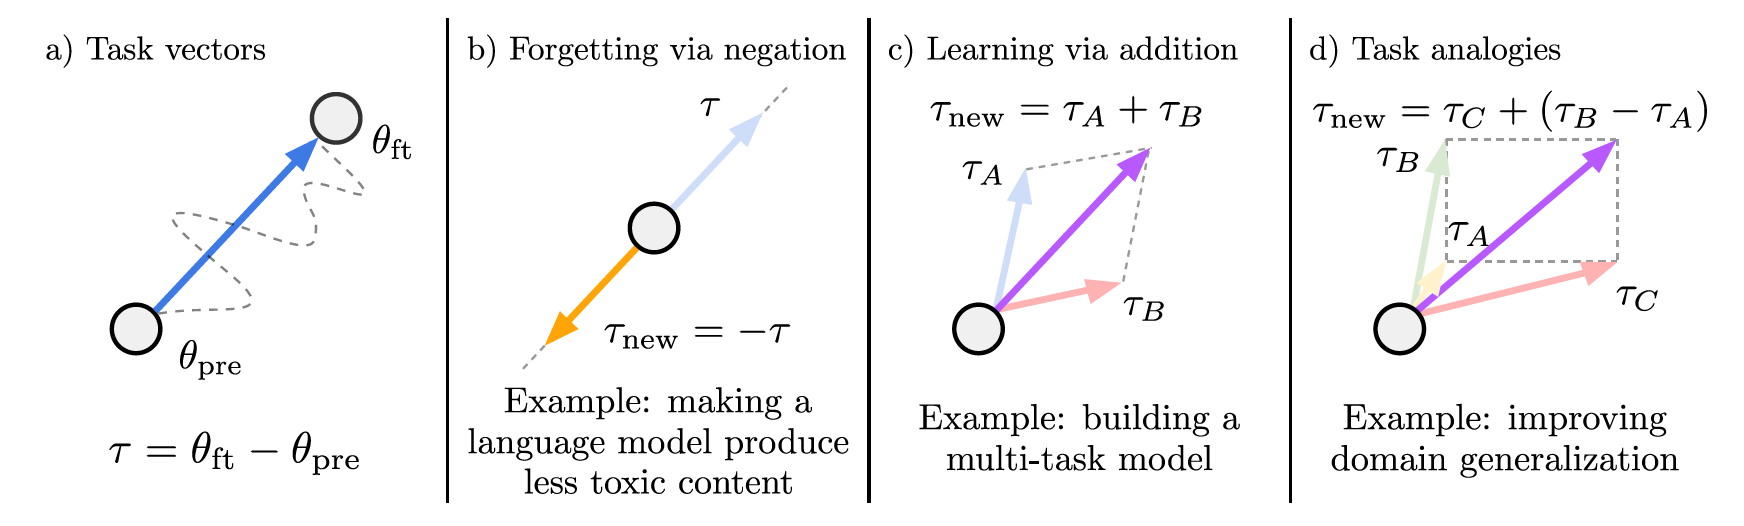
\includegraphics[width=\linewidth]{task-vector.png}
	\caption[Task vectors and their use in model editing]{Task vectors and their use in model editing: (a) A task vector is calculated by subtracting the weight parameters of a pre-trained model from the weights after it has been fine-tuned on a specific task. (b) By negating a task vector, the model's performance on a particular task can be reduced without significantly affecting its performance on unrelated tasks. (c) A model's capabilities on multiple tasks can be enhanced by summing up their respective task vectors. (d) Task vectors can also be manipulated through analogical relationships between tasks, allowing improvements in one task based on the relationships derived from others (\citet{ilharco2023editing}).}
	\label{fig:task-vector}
\end{figure}

\paragraph{Forgetting via Negation:} Forgetting or unlearning a specific task can be achieved by negating the task vector as shown in Figure \ref{fig:task-vector}(b). Negating a task vector \( \tau \) effectively reverses the direction of adjustment made by the original task training, thus degrading the model's performance on that task. Mathematically, this is represented as:
\begin{equation}
	\tau_{new} = -\tau
\end{equation}

This operation results in a model whose performance on the target task is decreased, with minimal impact on other tasks.

\paragraph{Learning via Addition:} Learning new tasks or improving performance on multiple tasks can be facilitated by the addition of task vectors as shown in Figure \ref{fig:task-vector}(c). When task vectors \( \tau_1, \tau_2, \ldots, \tau_n \) corresponding to different tasks are added, the resultant model is enhanced for all those tasks. The cumulative task vector is:
\begin{equation}
	\tau_{new} = \sum_{i=1}^n \tau_i
\end{equation}

Adding task vectors is especially effective for multitasking, allowing a single model to perform well across multiple tasks by leveraging the cumulative adjustments of each vector.

\paragraph{Task Analogies:} Task analogies as shown in Figure \ref{fig:task-vector}(d)  allow for the application of learned adjustments in new contexts, drawing on the analogy ``A is to B as C is to D". For tasks A, B, C, and D, if the task vectors for A, B, and C are known, the task vector for D can be approximated as:
\begin{equation}
\tau_D = \tau_C + (\tau_B - \tau_A)
\end{equation}

This approach utilizes differences and similarities across tasks to generalize to new tasks or domains without direct training data, effectively using transfer learning through task vector arithmetic.

\paragraph{Application:} One of the application of task-specific model editing is in multi-task learning, where adding multiple task vectors can enhance the model’s performance across several tasks simultaneously. This not only improves efficiency but also reduces the computational overhead associated with managing multiple distinct models. Furthermore, when tasks exhibit analogous relationships, combining appropriate task vectors can even improve performance on tasks for which the model has not been explicitly trained. This demonstrates the usefulness of this method in utilizing existing data to address data scarcity in new or related tasks.

\paragraph{Limitation} By applying simple arithmetic operations on these vectors—such as addition, subtraction, or negation, the model's behavior can be effectively edited as shown in Figure \ref{fig:task-vector}. However, there are also several limitations to consider:
\begin{itemize}
	\item \textbf{Architecture Dependency:} Task vectors are applicable only within models that share the same architecture. This is because task vectors involve element-wise operations on model weights, which assume a uniform structure across different model instances.
	\item \textbf{Same Pre-trained Initialization:} The effectiveness of task vector arithmetic is demonstrated under the condition that all models are fine-tuned from the same pre-trained initialization. This limits the applicability of task vectors since different initializations may lead to variations in how models learn and adapt, which could affect the applicability of the task vectors calculated from them.
	\item \textbf{Restriction to Linear Transformations}: The method primarily involves linear operations on task vectors. Non-linear interactions between model parameters or tasks may not be effectively captured or modified through simple vector arithmetic.
\end{itemize}

\section{Cross-Lingual Fact Representation}

\paragraph{Types of Fact Representation:} Multilingual Language Models (ML-LMs) employ various strategies for the representation of factual knowledge across languages. Factual knowledge in ML-LMs is represented in three distinct ways as proposed by \citet{zhao2024tracing}: language-independent, cross-lingual shared, and cross-lingual transferred.
\begin{itemize}
	\item \textbf{Language-Independent Representation:} This type of representation involves encoding factual knowledge using distinct neurons for each language. Each language has a unique set of neurons responsible for the representation of facts, independent of other languages. In some cases, the activity patterns of neurons differed when predicting the same fact in different languages. It means that the model's representation of this type of fact is not tied to any specific language as shown in Figure \ref{fig: fact}(a).
	
	\item \textbf{Cross-Lingual Shared Representation:} As shown in Figure \ref{fig: fact}(b), in the cross-lingual shared representation, ML-LMs use the same set of neurons to represent the same facts across multiple languages. This shared approach implies that a single neural configuration can encode factual knowledge in a way that is accessible and meaningful across different linguistic contexts, enhancing the model's ability to generalize across languages.
	
	\item \textbf{Cross-Lingual Transferred Representation:} This representation type involves transferring factual knowledge from one language to others, typically from a high-resource language to low-resource languages as shown in Figure \ref{fig: fact}(c). It is based on the fact that certain factual knowledge, once learned in one language, can be mapped onto other languages using a transformation of the learned representations. This method is particularly useful for efficiently scaling factual knowledge across languages in a model.
	
\end{itemize}

\begin{figure}[tbh]
	\centering
	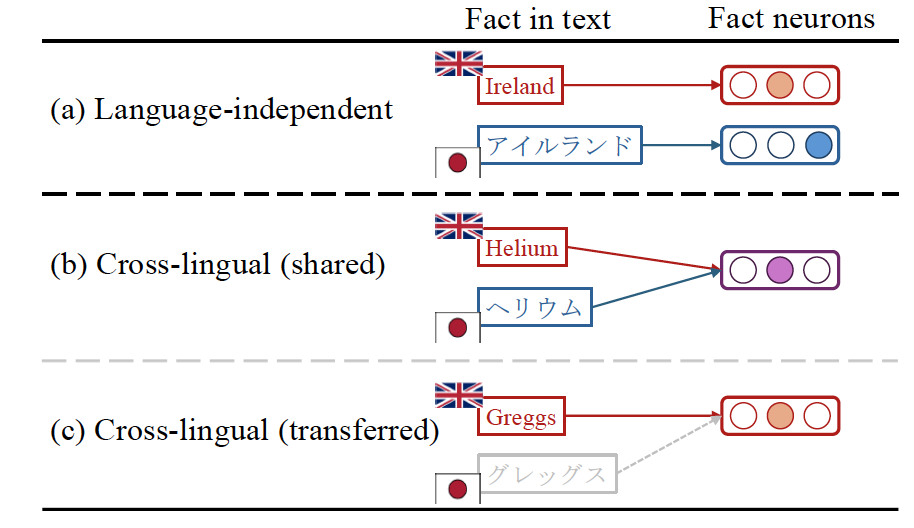
\includegraphics[width=0.75\textwidth]{fact}
	\caption[Cross-lingual fact representation]{Cross-lingual fact representation (b, c) -- same set of neurons are active for the same fact encoded in 2 different languages. Language independent representation (a) -- different set of neurons are active for the same fact encoded in 2 different languages (\citet{zhao2024tracing}).}
	\label{fig: fact}
\end{figure}

\paragraph{Effect of Training Data in Factual Probing:} It's challenging to estimate the amount of distinct factual knowledge present in the training data of multi-lingual LMs. It has been found that out of 3 metrics -- data-size of abstracts, number of page count and data-size of articles, the highest correlation (0.51) with P@1 is observed for data-size of abstracts. The precision tuple and data-size of abstracts tuple is shown in Figure \ref{fig: data-volume}.

\begin{figure}[tbh]
	\centering
	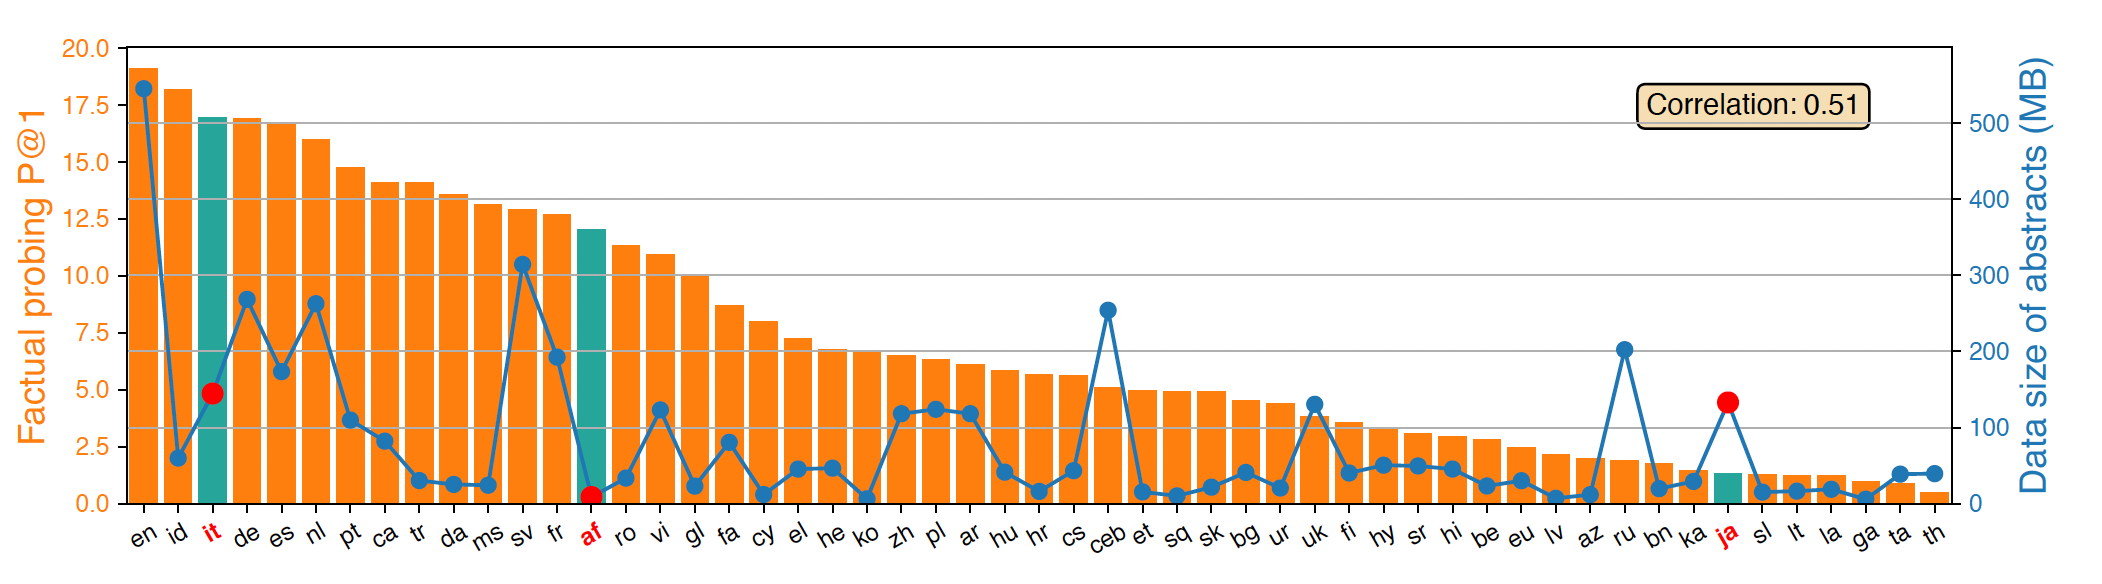
\includegraphics[width=\textwidth]{data-volume}
	\caption[P@1 score for factual probing results in m-BERT model with full match approach]{P@1 score for factual probing results in m-BERT model with full match approach. Italian and Japanese have P@1 score of 16.94\% and 1.34\% even though both of these languages are high resource with more than 100 MB of abstracts. This could be due to cultural biases in the mLAMA dataset, affecting non-Latin script languages (biases alone do not explain these substantial difference). Afrikaans language despite being low resource (\textless 20 MB), shows high precision score (12.05\%) for factual probing (\citet{zhao2024tracing}).}
	\label{fig: data-volume}
\end{figure}

\paragraph{Formation of Cross-Lingual Fact Representation:} Since the presence of cross-lingual fact representation is confirmed by neuron activity patterns by \citet{zhao2024tracing}, it is important to find out whether they are shared or transferred as shown in Figure \ref{fig: fact}. 
\begin{itemize}
	\item \textbf{Tracing of Roots:} The goal of \emph{tracing the roots of facts} is to check if a given fact originates from the training data (Wikipedia). To achieve this, string matching is performed between the object-subject pair and text (by WikiExtractor). If they co-occur, the fact is considered present, otherwise, it is considered as absent. These representations are identified through advanced probing methods using datasets like mLAMA, which consist of cloze-style queries designed to test the models' factual knowledge. 
	\item \textbf{Absent yet Predictable Facts:} This involves assessing whether m-BERT correctly predicts the presence or absence of certain facts, even if they are not verifiable in the training data. Many of the facts that were absent in the knowledge source but correctly predicted were relatively easy to predict because of entity tokens and naming cues as shown in Table \ref{T:naming-cues} and \ref{T:shared-entity}. The remaining facts other than entity tokens and naming cues are difficult to infer from the entities only, indicating the high possibility of cross-lingual transfer as shown in Table \ref{T:other}.
\end{itemize}

\begin{figure}[tbh]
	\centering
	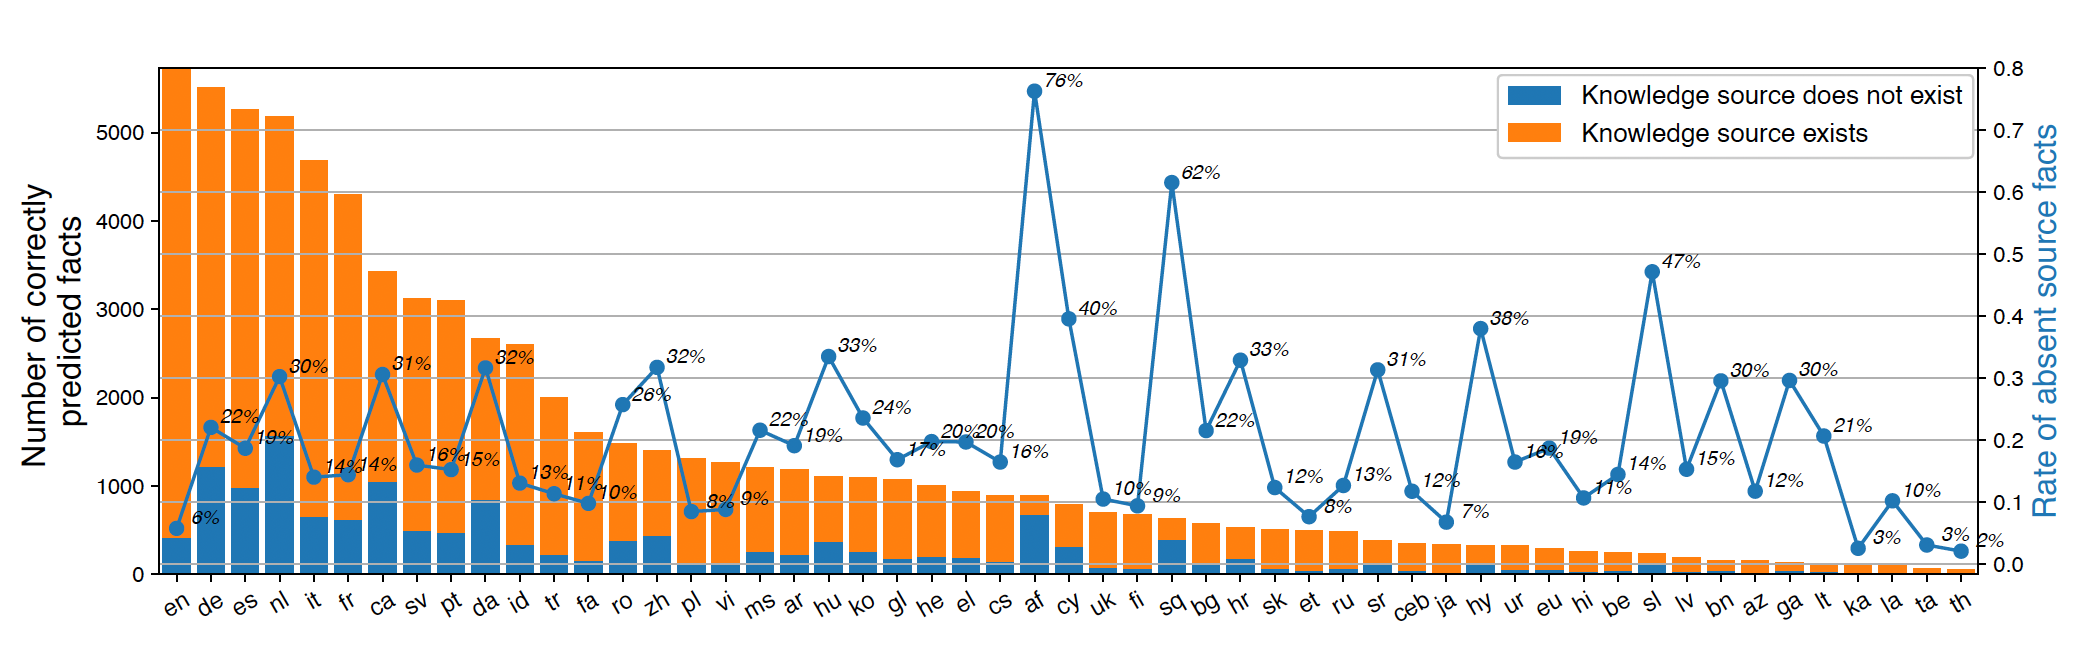
\includegraphics[width=\textwidth]{pred-fact}
	\caption[Number of correctly-predicted facts with mBERT in terms of existence of knowledge source]{Number of correctly-predicted facts with mBERT in terms of existence of knowledge source: As more training data leads to a more comprehensive understanding of language and its associated facts, it is observed that languages with larger training data tend to have better coverage of factual knowledge as anticipated. However, facts in low resource languages like Afrikaans and Albanian are correctly predicted despite not being verifiable in the training corpus indicating a high possibility of effective cross-lingual transfer (\citet{zhao2024tracing}).}
	\label{fig: pred-fact}
\end{figure}

\begin{table}[tbh!]
	\centering
	\begin{tabular}{c c c}
		\hline
		\textbf{Language} & \textbf{Absent yet predictable facts} & \textbf{Naming cues} \\
		\hline
		English & \texttt{The native language of Hamidou is French.} & \texttt{Hamidou} \\
		Spanish & \texttt{Bruno solia comunicarse en frances.} & \texttt{Bruno} \\
		\hline
	\end{tabular}
	\caption{Examples of easy-to-predict facts using naming cues}
	\label{T:naming-cues}
\end{table}

\begin{table}[tbh!]
	\centering
	\begin{tabular}{c c c}
		\hline
		\textbf{Language} & \textbf{Absent yet predictable facts} & \textbf{Entity tokens} \\
		\hline
		English & \texttt{Sega Sports R\&D is owned by Sega} & \texttt{Sega} \\
		Spanish & \texttt{Honda Express es producido por Honda.} & \texttt{Honda} \\
		\hline
	\end{tabular}
	\caption{Examples of easy-to-predict facts using entity tokens.}
	\label{T:shared-entity}
\end{table}

\begin{table}[tbh!]
	\centering
	\begin{tabular}{c c}
		\hline
		\textbf{Language} & \textbf{Absent yet predictable facts}  \\
		\hline
		English & \texttt{Aleksandar Novakovic was born in Belgrade} \\
		Spanish & \texttt{Aleksandar Novakovic nacio en Belgrado} \\
		\hline
	\end{tabular}
	\caption{Examples of non-easy-to-predict facts.}
	\label{T:other}
\end{table}
	
\paragraph{Limitations:} The probing results often reveal that while ML-LMs are capable of recalling facts in high-resource languages, their performance in low-resource languages can be inconsistent, primarily due to limited training data and potential cultural biases in the datasets. Despite its advantages, cross-lingual fact transfer faces challenges such as:
\begin{itemize}
	\item \textbf{Inconsistency Across Languages:} The transfer process might not always maintain accuracy due to linguistic and cultural differences.
	\item \textbf{Reliance on Source Languages:} The success of the transfer often depends heavily on the data quality and availability in the source languages.
	\item \textbf{Complex Representations:} The complexities involved in how different languages structure factual information can limit the effectiveness of the transfer.
\end{itemize}

\section{Geometry of Language Model Representation}
\paragraph{Language Subspace and Axes:} Recent studies, such as those conducted by \citet{chang2022geometry}, have explored how multilingual models like XLM-R maintain shared multilingual spaces while encoding language-sensitive information. Their findings illustrate that languages tend to occupy similar linear subspaces in high-dimensional embedding spaces, especially after processes like mean-centering, which aligns the subspaces by adjusting for language-specific offsets in the representation mean. The space contains embeddings or vectors assigned to tokens based on their semantic or syntactic properties. Subspaces are low-dimensional vector space within the high-dimensional embedding space that capture certain linguistic properties. Mean-centering involves subtracting the mean (over all subspace vectors) from each data point within a subspace. The language sensitive axes are axes (basic vectors) that are within the subspace that capture language-specific information (e.g. grammar). The language neutral axes are axes that are within the subspace encode information that is common across languages, such as word position or parts of speech.

\paragraph{Identification of subspace by SVD:} For a particular \emph{language A}, 512 input sentences are taken(each consists of 512 tokens) --- therefore giving a total 262K contextual tokens.
\begin{equation}
	\mathbf{c}^{(i)} \in \mathbb{R}^d \text{ where } i \in \{1, 2, \dots , 262K\}
\end{equation}

The mean context vector and data covariance matrix can be calculated as:
\begin{equation}
	\bm{\mu}_A = \frac{1}{262K}\sum_{i=1}^{262K} \mathbf{c}^{(i)} \in \mathbb{R}^d
\end{equation}
\begin{equation}
	S = \frac{1}{262K} \sum_{i = 1}^{262K} (\mathbf{c}^{(i)} - \bm{\mu}_A)(\mathbf{c}^{(i)} - \bm{\mu}_A)^T \in \mathbb{R}^{d \times d}
\end{equation}

After performing the eigenvalue decomposition on $S$, the top $k$ (corresponding to largest $k$ eigenvalues) eigenvectors of $S$ are given by $V_A \in \mathbb{R}^{d \times k}$. The language subspace is identified by k eigenvector of $S$. \citet{chang2022geometry} selected $k$ such that $q/p = 0.9$. Considering the eigenvalues sequence of $S$ in decreasing order as $E$, the ratio $q/p$ can be calculated as follows:
\begin{equation}
	E = (\lambda_1, \lambda_2, \dots , \lambda_d) \text{ s.t. } \lambda_i \ge \lambda_{i+1} \quad \forall i \in \{1,2, \dots, d\}
\end{equation}
\begin{align}
	q &= \sum_{i = 1}^{k} E[i]\\
	p &= \sum_{i=1}^{d} E[i]
\end{align}

The dimension of the context vector $d$ was originally 768 and if the value of reduced dimension $k$ is considered from each of the 12 layers of the transformer then the median value of $k$ was found to be 335.

\paragraph{Perplexity Ratio:} From the LLM, the token $\mathbf{t}^{(i)}$ is predicted given the previous sequence of tokens $(\mathbf{t}^{(j)})_{j = 1}^{j = i-1}$. Suppose the LLM predicts the token $\mathbf{t}^{(i)}$ with probability $\mathbb{P}(\mathbf{t}^{(i)} \mid \mathbf{t}^{(i-1)}, \dots , \mathbf{t}^{(1)})$. Then the perplexity of the LLM would be defined as:
\begin{equation}\label{E:pp}
	pp(\mathbf{t}^{(i)}, \mathbf{t}^{(i-1)}, \dots , \mathbf{t}^{(1)}) = \prod_{i = 1}^{N} \left[ \frac{1}{\mathbb{P}(\mathbf{t}^{(i)} \mid \mathbf{t}^{(i-1)}, \dots , \mathbf{t}^{(1)})} \right]^{\frac{1}{N}}
\end{equation}

Suppose $\mathbf{x}$ is a word vector which originally belongs to \emph{language A}. Then projection of $\mathbf{x}$ after mean centering onto the language subspace of A gives $\mathbf{u}$. Again projecting this vector $\mathbf{u}$ onto the model space, the reconstructed word vector $\hat{\mathbf{x}}$ is obtained as:
\begin{align}
	\mathbf{u} &= V_A^T(\mathbf{x} - \bm{\mu}_A) \\
	\hat{\mathbf{x}} &= V_A V_A^T (\mathbf{x} - \bm{\mu}_A) + \bm{\mu}_A
\end{align}

The perplexity of the LLM (with Equation \ref{E:pp}) for all the languages represented in the original model space would be calculated as follows:
\begin{align}
	\text{Language-A:}& \quad \mathbf{x}_A^{(i)[l]} \quad \forall i \in \{1, 2, \dots, N\},\; \forall l \in \{1, 2, \dots, 12\} \Longrightarrow pp_A^{[l]} 
\end{align}

The perplexity of the LLM (with Equation \ref{E:pp}) for all the languages reconstructed from the language subspace would be calculated as follows:
\begin{align}
	\text{Language-A:}& \quad \hat{\mathbf{x}}_A^{(i)[l]} = V_A^{[l]} V_A^{[l]^T} (\mathbf{x}_A^{(i)[l]} - \bm{\mu}_A^{[l]}) + \bm{\mu}_A^{[l]}  \quad \forall i, \; \forall l \Longrightarrow \hat{pp}_{A}^{[l]}
\end{align}

The perplexity ratio for each of the layer and for each of the language would be calculated as follows:
\begin{align}
	\text{Language-A:}& \quad r_A^{[l]} = \frac{\hat{pp}_A^{[l]}}{pp_A^{[l]}} \quad \forall l \in \{0, 1, \dots , 12\}
\end{align}

The average perplexity ratio over all the 88 languages for each of the layer would be calculated as follows:
\begin{equation}
	r^{[l]} = \frac{1}{88} \sum_{i = A}^{CJ} r_i^{[l]} \quad \forall l \in \{0, 1, \dots , 12\}
\end{equation}

\paragraph{Justification -- Affine subspaces can be used for language modeling:}
\begin{itemize}
	\item To reconstruct the vectors of a particular \emph{language A} from its corresponding \emph{language subspace A}, the following equation can be used.
	\begin{equation}\label{E:Proj_A}
		Proj_A(\mathbf{x}_A) = V_A V_A^T (\mathbf{x}_A - \bm{\mu}_A) + \bm{\mu}_A 
	\end{equation}
	
	\item From Figure \ref{F:proj} ($Proj_A$ curve), it is clear that when the vectors are reconstructed as per Equation \ref{E:Proj_A} then the perplexity (calculated by $Proj_A(\mathbf{x}_A)$) does not increase significantly as compared to the no projection perplexity (calculated by $\mathbf{x}_A$).
	
	\item This suggests that the information necessary for language modeling task for a particular \emph{language A} is well-preserved within the lower-dimensional \emph{language subspace A}.
	
\end{itemize}

\begin{figure}[tbh]
	\centering
	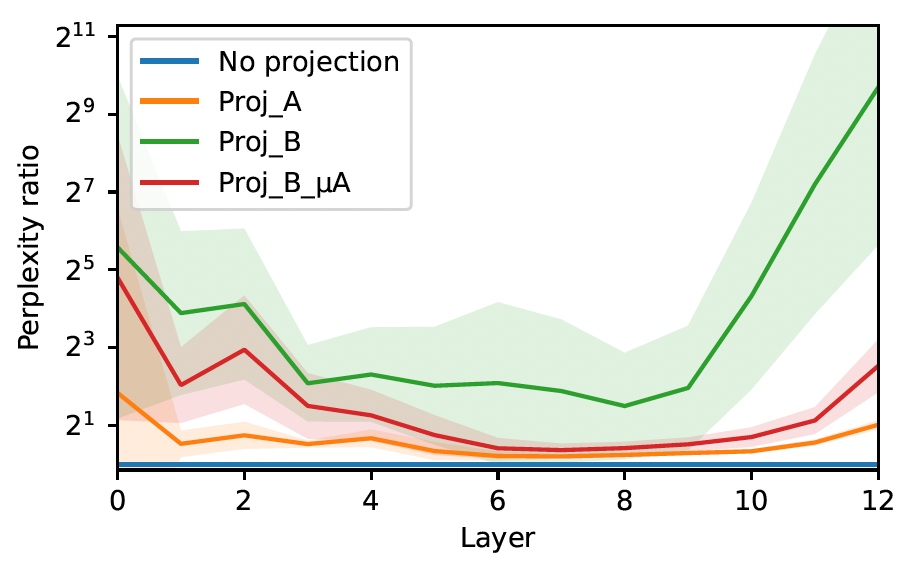
\includegraphics[width=0.8\textwidth]{proj}
	\caption[Variation of perplexity ratio at different transformer layers of LLM]{Variation of perplexity ratio at different transformer layers of LLM. (\citet{chang2022geometry})}
	\label{F:proj}
\end{figure}

\paragraph{Justification -- Language subspaces differed from one another:}
\begin{itemize}
	\item To reconstruct the vectors of a particular \emph{language A} from another \emph{language subspace B}, the following equation can be used.
	\begin{equation}\label{E:Proj_B}
		Proj_B(\mathbf{x}_A) = V_B V_B^T (\mathbf{x}_A - \bm{\mu}_B) + \bm{\mu}_B
	\end{equation}
	
	\item From Figure \ref{F:proj} ($Proj_B$ curve), it is clear that when the vectors are reconstructed as per Equation \ref{E:Proj_B} then the perplexity (calculated by $Proj_B(\mathbf{x}_A)$) increases significantly as compared to the no projection perplexity (calculated by $\mathbf{x}_A$).
	
	\item This indicates that the \emph{language subspace B} is not suitable for representing text in \emph{language A}. This implies that the model has learned to differentiate between languages.
\end{itemize}

\paragraph{Justification -- Mean-shifted subspaces were similar to one another:}
\begin{itemize}
	\item To reconstruct the vectors of a particular \emph{language A} after mean centering from another \emph{language subspace B}, the following equation can be used.
	\begin{equation}\label{E:Proj_B_mu_A}
		Proj_{B, \bm{\mu}_A}(\mathbf{x}_A) = V_B V_B^T (\mathbf{x}_A - \bm{\mu}_A) + \bm{\mu}_A
	\end{equation}
	
	\item From Figure \ref{F:proj} ($Proj_{B, \bm{\mu}_A}$ curve), it is clear that when the vectors are reconstructed as per Equation \ref{E:Proj_B_mu_A} then the perplexity (calculated by $Proj_{B, \bm{\mu}_A}$) does not increase significantly as compared to the no projection perplexity (calculated by $\mathbf{x}_A$).
	
	\item Projecting onto the affine subspace for \emph{language B} but shifted as per its own language mean was similar to projecting onto the affine subspace for its own \emph{language A}. This means, the affine subspaces for different languages are similar to one another when shifted according to language means.
\end{itemize}

\paragraph{Geometric Insights:} One of the key insights from this research is the identification of patterns and shapes such as spirals, toruses, and curves within these subspaces, which represent different types of linguistic information as shown in Figure \ref{fig: geometry-insight}. For example, token position information forms a nearly perfect torus in the projected subspace, suggesting a geometric encoding of sequential information that is consistent irrespective of the language. These geometric insights by \citet{chang2022geometry} enable more targeted approaches to model training and fine-tuning, where language-specific and task-specific adjustments can be made based on the geometric properties of the model's representational space. This can potentially lead to improvements in model efficiency and effectiveness, particularly in tasks involving multiple languages.

\begin{figure}[tbh]
	\centering
	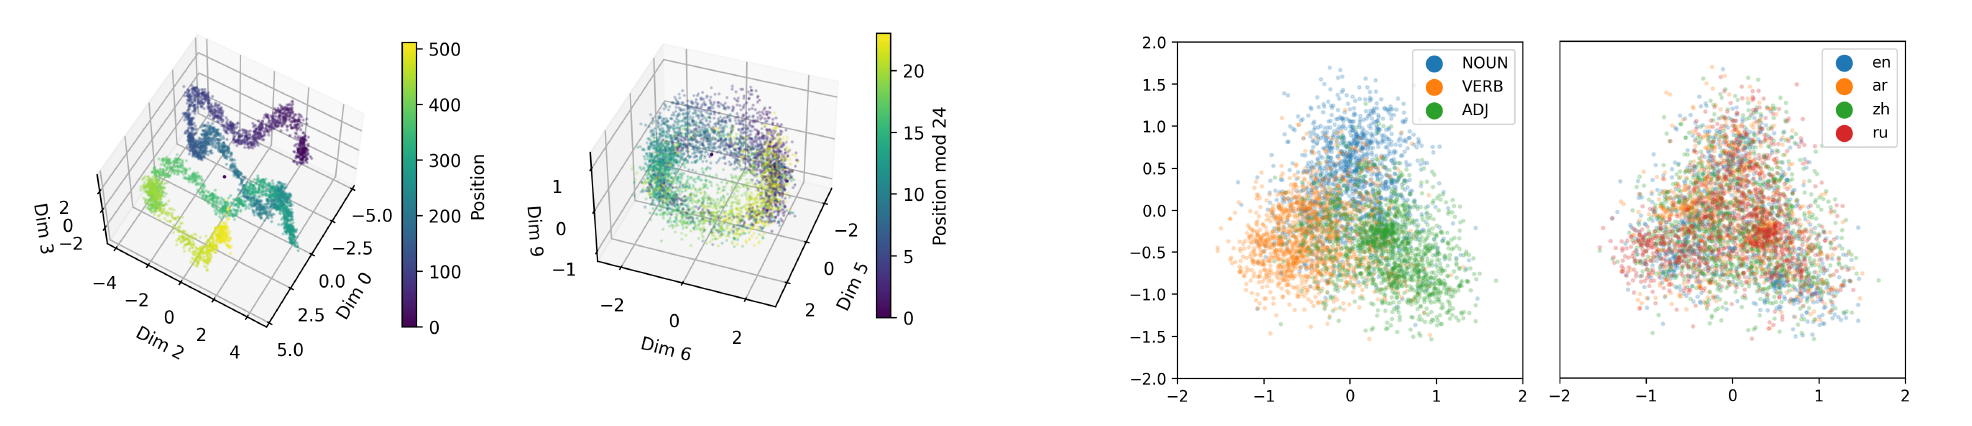
\includegraphics[width=\textwidth]{geometry-insight}
	\caption[Geometric insights of tokens]{Geometric insights: (Left) shows the geometric representation of token positions in layer four of the XLM-R model, illustrating absolute positions with curves and relative positions with toruses. (Right) depicts the clustering of nouns, verbs, and adjectives in layer two, highlighting the model's ability to distinguish and generalize part-of-speech categories across different languages. (\citet{chang2022geometry})}
	\label{fig: geometry-insight}
\end{figure}

\paragraph{Limitations:} Despite its insights, the study acknowledges several limitations that could impact the generalizability of the findings:
\begin{itemize}
	\item The linguistic diversity in the dataset is skewed towards Indo-European languages, which may not accurately represent the behavior of the model across globally diverse languages.
	\item Variations in corpus size and quality across different languages could lead to disparities in the learned representations, potentially biasing the model's performance towards languages with richer data resources.
	\item The study's reliance on a single model architecture (XLM-R) may limit the applicability of the findings to other multilingual models with different architectures.
\end{itemize}
